\documentclass[10pt]{article}
\usepackage{pictex,amsmath,amssymb,amsfonts,amsthm,verbatim}
\usepackage{graphics}
\usepackage{fullpage}
\usepackage{fancyhdr}
\usepackage{algorithm,algorithmic}
\usepackage{multirow}
\usepackage{gensymb}
\usepackage{graphicx}
\usepackage{mathrsfs}

\setlength{\voffset}{-0.25in}
\setlength{\headsep}{+0.5in}
\setlength{\parskip}{1em}
\setlength{\parindent}{0em}

\def\vu{\mathbf{u}}
\def\vv{\mathbf{v}}
\def\vb{\mathbf{b}}
\def\vw{\mathbf{w}}
\def\vs{\mathbf{s}}

\renewcommand{\implies}{\rightarrow}
\renewcommand{\lor}{\vee}
\renewcommand{\land}{wedge}
\renewcommand{\iff}{\leffrightarrow}
\newcommand{\TRUE}{\mathbf{T}}
\newcommand{\FALSE}{\mathbf{F}}
\newcommand{\universe}{\mathcal{U}}

\usepackage{xcolor}
\usepackage{titlesec}
\usepackage{mdframed}
\usepackage{amsmath}
\usepackage[utf8]{vietnam}

\newmdenv[linecolor=blue,skipabove=\topsep,skipbelow=\topsep,leftmargin=5pt,rightmargin=-5pt,innerleftmargin=5pt,innerrightmargin=5pt]{mybox}

\begin{document}
\begin{center}
\textbf{TEMPERATURE}
\end{center}
\begin{enumerate}
	%1
	\item \textbf{Temperature and the Zeroth Law of Thermodynamics}
	\begin{itemize}
		\item \textbf{Thermal equilibrium} is the situation in which two objects would not exchange energy by heat or electromagnetic radiation if they were placed in thermal contact.
		\item \textbf{The zeroth law of thermodynamics} :If odjects A and B are separately in thermal equilibrium with object C, then A and B are in thermal equilibrium with each other.
	\end{itemize}
	%2
	\item \textbf{Thermometers and the Celsius Temperature Scale}\\
	- Thermometer is the devices that are used to measure the temperature of a system.\\
	- All thermometer are based on the principle that some physical property of a system changes as the temperature changes.Some physical properties is (1) the volume of a liquid, (2) the dimensions of a solid, (3) the pressure of a gas at constant volume, (4) the volume of a gas at constant pressure, (5) the electric resistance of a conductor, (6) the color of an object\\
	- A common thermometer in  everyday use consist of a mass of liquid -- usually mercury or alcohol.\\
	- \textbf{The Celsius temperature scale} uses the mixture of water and ice in thermal equilibrium at atmospheric pressure, this mixture is defined to have a temperature of zero degrees Celsius, which are writen as 0 \degree C, which is called as the ice point of water. another is defined as the steam point of water, which is written as 100 \degree C.
	%3
	\item \textbf{The absolute temperature scale} (\degree K)
	\begin{mybox}
	\begin{center}
	$T_C = T - 273.15$
	\end{center}
	\end{mybox}
	- So, the ice-point temperature on the Kelvin scale is 273.15 \degree, corresponds to 0 \degree C, and the Kelvin steam point is 373.15 \degree, is equivalent to 100 \degree C
	%4
	\item \textbf{The Fahrenheit scale}
	\begin{mybox}
	\begin{center}
	$T_f = \dfrac{9}{5}T_c + 32 \degree F$
	\end{center}
	\end{mybox}
	\textbf{The relation between changes in temperature on the Celsius, Kelvin, and Farenheit scales:}
	\begin{mybox}
	\begin{center}
	$\Delta T_C = \Delta T = \dfrac{5}{9} \Delta T_F$
	\end{center}
	\end{mybox}
	%5
	\item \textbf{Thermal Expansion of Solids and Liquids}\\
	- \textbf{Thermal Expansion} is a consequence of the change in the average separation between the atoms in the subject\\ 
	- As the temperature of the solid increases, the atoms oscilate with greater amplitudes; as a result, the average separation between them increases. Consequently, the object expands.\\
	\textbf{The average coefficient of linear expansion:}
	\begin{mybox}
	\begin{center}
	$\alpha = \dfrac{\Delta L / L_i}{\Delta T}$
	\end{center}
	\end{mybox}
	\pagebreak
	- Because the linear expansion of an object change with temperature also susrface area and volume change as well.So:
	\begin{mybox}
	\begin{center}
	$\Delta V = \beta V_i \Delta T$
	\end{center}
	\end{mybox}
	Where $\beta$ is the average coefficient of volume expansion.\\
	For a solid, $\beta = 3 \alpha$.
	%6
	\item \textbf{Ideal Gas}
	\textbf{Equation state of Ideal Gas}
	\begin{mybox}
	\begin{center}
	PV=nRT
	\end{center}
	\end{mybox}
	\begin{itemize}
	\item for R = 8.314 J/mol $\cdot K$\\
	 	$P:Pa(N/m^2)$\\
	 	$V:m^3$\\
	\item for R = 0.08214 L $\cdot atm/mol \cdot K$\\
	    P:atm\\
	    $V:L(1L = 10^3 cm^3 = 10^{-3} m^3)$\\
	\end{itemize}
	%7
	\item \textbf{Boltzman's constant}
      \begin{mybox}
	\begin{center}
	PV = nRT = $\dfrac{N}{N_A} RT$\\
       \end{center}
       \end{mybox}
	$\rightarrow{PV = Nk_BT}$
	For $k_B = \dfrac{R}{N_A} = 1.38 \times 10^{-23} J/K$ 
\end{enumerate}
\pagebreak
\begin{center}
\textbf{HEATS AND THE FIRST LAW OF THERMODYNAMICS}
\end{center}
\begin{enumerate}
	%1
	\item \textbf{Heat and Internal Energy}\\
	- \textbf{Internal energy} (Nội năng) is all the energy of a system that is associated with its microscopic components -atoms and molecules-when viewd from a reference frame at rest with respect to the center of mass of the system.\\
	- \textbf{Heat} (Nhiệt lượng) is defined as the transfer of energy across the boundary of a system due to a temperature difference between the system and its surroundings.\\
	%2
	\item \textbf{Unit of Heat}\\
	- Calorie(Cal) is defined as the amount of energy transfer necessary to raise the temperature of 1g of water from 14.5 \degree C to 15.5 \degree C
	\begin{mybox}
	\begin{center}
	1 Calorie = $1.00 \times 10^3 cal$
	\end{center}
	\end{mybox}
	%3
	\item \textbf{The Mechanical Equivalent of Heat}
	\begin{mybox}
	\begin{center}
	1 cal = 4.186J
	\end{center}
	\end{mybox}
	For the work done is equivalent to the calories release is:
	\begin{mybox}
	\begin{center}
	W = nmgh
	\end{center}
	\end{mybox}
	With:\\
	n = the work done in \textbf{n} times.\\
	m = mass of an object.\\
	%4
	\item \textbf{Specific Heat and Calorimetry}\\
	- The \textbf{heat capacity} (nhiệt dung) \textbf{C} of a particular sample of a substance is defined as the amount of energy needed to raise the temperature of that sample by 1 \degree C.
	\begin{mybox}
	\begin{center}
	$Q = C \Delta T$
	\end{center}
	\end{mybox}
	- The \textbf{specific heat} (nhiệt dung riêng) \textbf{c} of a substances is the heat capacity per unit mass.
	\begin{mybox}
	\begin{center}
	$c = \dfrac{Q}{m \Delta T}$
	\end{center}
	\end{mybox}
      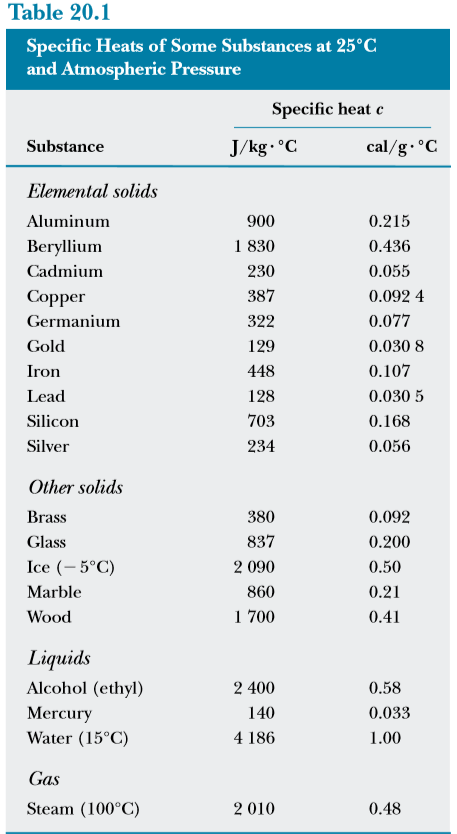
\includegraphics{Hinh2}\\  
	\textbf{Conversation of Energy:Calorimetry}\\
	- One tecnique for measuring specific heat involves heating the sample to temperature $T_X$ and place it in a vessel of water that $T_{water} < T_X$ and measure the temperature of water after equilibrium is \textbf{calorimetry} (phép đo nhiệt lượng), and the device is used where the energy transfers occured is \textbf{calorimeter}.\\
	- If the system of sample and the water is isolated , the law of the converational of energy requires the amount of energy that \textbf{leaves} the sample is \textbf{equal} to the amount of energy that \textbf{enters} the water.\\
	\begin{mybox}
	\begin{center}
	$Q_{cold} = -Q_{hot}$
	\end{center}
	\end{mybox}
      The \textbf{sum} of energy transferred is zero.
      \begin{mybox}
      \begin{center}
      $Q_1 + Q_2 + Q_3 + \cdots +Q_N = 0$
      \end{center}    
      \end{mybox}    
	In this situation:
	\begin{center}
	$m_{water}c_{water}(T_f-T_i) > 0 \mbox{ as }(T_f > T_i)$\\
	$m_Xc_X(T_f-T_i) <0 \mbox{ as } (T_f < T_i)$\\
	\end{center}
	Then:
	\begin{mybox}
	\begin{center}
	 $m_{water}c_{water}(T_f-T_i) = -m_Xc_x(T_f-T_i)$
	 \end{center}
	 \end{mybox}
	 %5
	 \item \textbf{Latent Heat}\\
	 - In some situations the change of energy transfer does not result in the change of temperature, it is commonly referred as a \textbf{phase change}\\
	 - There are three common \textbf{phase change}:\\
	  + Solid to liquid.\\
	  + Liquid to gas.\\
	  + Crystalline structure of a solid.\\
	 - Such \textbf{phase changes} involve a change in internal energy but no change in temperature.\\
	\begin{mybox}
	\begin{center}
	$Q = \pm mL$
	\end{center}
	\end{mybox}
	%6
	\item \textbf{Work and Heat in Thermodynamic Process}
	\begin{mybox}
	\begin{center}
	$W = - \int_{V_i}^{V_f}PdV$
	\end{center}
	\end{mybox}
	\begin{center}
	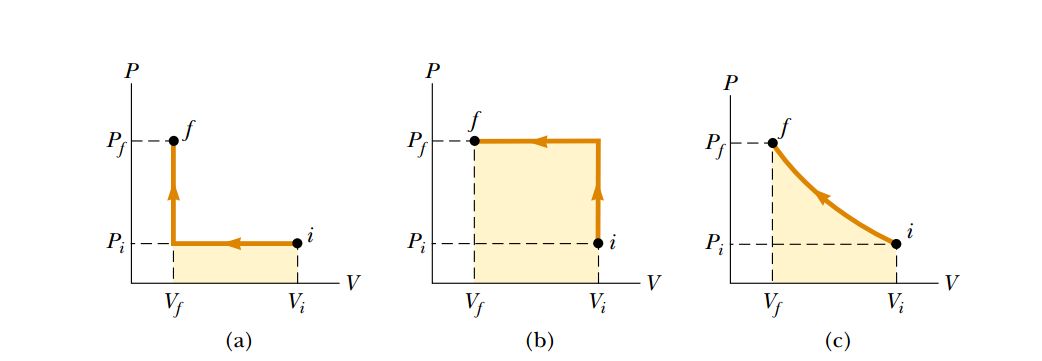
\includegraphics{hinh}
	\end{center}
	We can see from the picture that:\\
	$(a) W= -P_i(V_f-V_i)$\\
	$(b) W= -P_f(V_f-V_i)$\\
	$(c) W= W = - \displaystyle \int_{V_i}^{V_f}PdV$.\\
	%7
	\item \textbf{The first law of Thermodynamic}\\
	- The change in total energy of a system (also in the change of internal energy) is the work done on it plus the heat transferred.
	\begin{mybox}
	\begin{center}
	$\Delta E = \Delta U = Q + W$
	\end{center}
	\end{mybox}
	If:\\
	Q > 0; W > 0:receive thermal.\\
	Q < 0; W < 0:release thermal.\\
	%8
	\item \textbf{Applications of the First law of Thermodynamics}\\
	\begin{itemize}
		\item \textbf{An andiabatic process} (Q = 0) (Quá trình đoạn nhiệt): no energy enter or leaves the system by heat.
		\begin{mybox}
		\begin{center}
		$\Delta E = \Delta U = W + 0 = W$
		\end{center}
		\end{mybox}
		\item \textbf{An isovolumetric process} (Quá trình đẳng tích):V is constant
		\begin{mybox}
		\begin{center}
		$\Delta E = \Delta U = Q$
		\end{center}
		\end{mybox}
		\item \textbf{Isobaric process} (Quá trình đẳng áp):P is constant.\\
		\textbf{Tip:} The done by pressure is \textbf{F = PA}, for \textbf{A} is area.
		\begin{mybox}
		\begin{center}
		$W = -P(V_f-V_i)$
		\end{center}
		\end{mybox}
	\end{itemize}
	%9
	\item \textbf{Isothermal Expansion of an Ideal Gas}\\
	Because the gas is ideal and the process is quasi-static, we can use: 
	\begin{mybox}
	\begin{center}
	PV=nRT
	\end{center}
	\end{mybox}
	\begin{center}
	$W = - \displaystyle \int_{V_i}^{V_f}PdV = - \int_{V_i}^{V_f} \dfrac{nRT}{V}dV$
	\end{center}
	Evaluate the integral, we have:
	\begin{mybox}
	\begin{center}
	W = nRT ln($\dfrac{V_i}{V_f}$)
	\end{center}
	\end{mybox}
	%10
	\item \textbf{Energy Transfer Mechanisms}\\
	\textbf{Thermal Conduction} (Page 623)\\
	\begin{mybox}
	\begin{center}
	$\mathcal{P} = kA \displaystyle | \dfrac{dT}{dx} |$
	\end{center}
	\end{mybox}
	\textbf{Radiation} (Page 628)\\
	\begin{mybox}
	\begin{center}
	$\mathcal{P} = \sigma AeT^4$
	\end{center}
	\end{mybox}
\end{enumerate}
\pagebreak
\begin{center}
\textbf{THE KINETIC THEORY OF GASES}
\end{center}
\begin{enumerate}
	%1
	\item \textbf{Molecular Model of an Ideal Gas}
	\begin{itemize}
		\item The number of molecules in the gas is large, and the average separation between them is large compared with their dimensions
		\item The molecules obey Newton's laws of Motion, but as whole they move randomly.
		\item The molecules interact only by short-range forces during elastic collisions
		\item The molecules make elastic collisions with the walls
		\item The gas under consideration is a pure substance; that is, all molecules are identical.
	\end{itemize}
	%2
	\item \textbf{The basic equation of kinetic energy of an ideal gas}
	\begin{mybox}
	\begin{center}
	$PV = \dfrac{2}{3}N(\dfrac{1}{2}m \overline{v^2}) = \dfrac{2}{3}N \overline{K}$
	\end{center}
	\end{mybox}
	Beside: 
	\begin{mybox}
      \begin{center}
	$PV = Nk_BT$
      \end{center}  
	\end{mybox}
	%3
	\item \textbf{The average translational kinetic energy}
	\begin{mybox}
	\begin{center}
	$\overline{K} = \dfrac{3}{2}k_BT$
	\end{center}
	\end{mybox}
	\begin{center}
	$\rightarrow{\overline{v^2} = \dfrac{3k_BT}{m}}$
	\end{center}
	%4
	\item \textbf{Adiabatic Process for an Ideal Gas} (Page 649)
	\begin{mybox}
	\begin{center}
	$PV^{\gamma} = constant$
	\end{center}
	\end{mybox}
	%5
	\item \textbf{The Equiparition of Energy} (Sự phân bố đồng đều về năng lượng)\\
	- Each atom has three different motion:translational motion (chuyển động tịnh tiến), rotational motion, vibrationnal motion to create the degree of freedom.\\
	\textbf{Internal Energy of Ideal Gas}
	\begin{mybox}
	\begin{center}
	$U = (i_T + i_R + 2i_V) \dfrac{Nk_BT}{2}$
	\end{center}
	\end{mybox}
	%6
	\item \textbf{Boltzman Distribution}\\
	- All molecules are not average.\\
	- Each molecule has its own v.
	%7
	\item \textbf{Maxwell Distribution}\\
	\begin{itemize}
		\item  \textbf{The root-mean-square speed:}
		\begin{mybox}
		\begin{center}
		$v_{rms} = \sqrt{\overline{v^2}} = \sqrt{\dfrac{3k_BT}{m}}$
		\end{center}
		\end{mybox}
		\item \textbf{The average speed:}
		\begin{mybox}
		\begin{center}
		$\overline{v} = \sqrt{\dfrac{8k_BT}{m}}$
		\end{center}
		\end{mybox}
		\item \textbf{The most probable speed:}
		\begin{mybox}
		\begin{center}
		$v_{p}= \sqrt{\dfrac{2k_BT}{m}}$
		\end{center}
		\end{mybox}
	\end{itemize}		
\end{enumerate}
\pagebreak
\begin{center}
\textbf{HEATS ENGINES, ENTROPY, AND THE SECOND LAW OF THERMODYNAMICS}
\end{center}
\begin{enumerate}
	%1
	\item \textbf{Heat engines and the Second Law of Thermodynamics}.\\
	- A \textbf{heat engine} is the device that produce energy by means of work used coal and some fuels burnt.\\
	- The work done by engine is $Q_{eng}$, for the work done by heat engine is equal the net energy $Q_{net}$ transffered to it.
	\begin{mybox}
	\begin{center}
	$Q_{eng} = Q_{net} = |Q_h| - |Q_c|$
	\end{center}
	\end{mybox}
	- The \textbf{thermal efficiency} e of a heat engine is defined by the engine during one cycle to the energy input at the higher temperature
	\begin{mybox}
	\begin{center}
	$e = \dfrac{W_{eng}}{|Q_h|} = \dfrac{|Q_h| - |Q_c|}{|Q_h|} = 1 - \dfrac{|Q_c|}{|Q_h|}$
	\end{center}
	\end{mybox}
	From the equation, we consider that the efficiency of the heat engine wil be 100 \% only when e = 1 $\leftrightarrow{Q_c = 0}$, which means the engine always in hot situation without energy transferring between hot and cold reservoirs.\\
	\textbf{Kelvin-Planck form of the second law of Thermodynamics:}\\
	     \textit{It is impossible to construct a heat engine that, operating in a circle, produces no effect other than the input of energy by heat from the reservoir and the performance of an equal amount of work.}
	\textbf{Clausius statement:}
	     \textit{It is impossible to construct a cyclical machine whose sole effect is to transfer energy continously by heat from one object to another object at a higher temperature \textbf{without} the input of energy by work.}      
	%2
	\item \textbf{Heat Pumps and Refrigerators}\\
	\textit{The direction of heat always tranfers from hot reservoir to cold reservoir}.\\
	- In the refrigerator or heat pumps the engine take energy from cold reservoir to hot reservoir only exist the work done on the engine.\\
	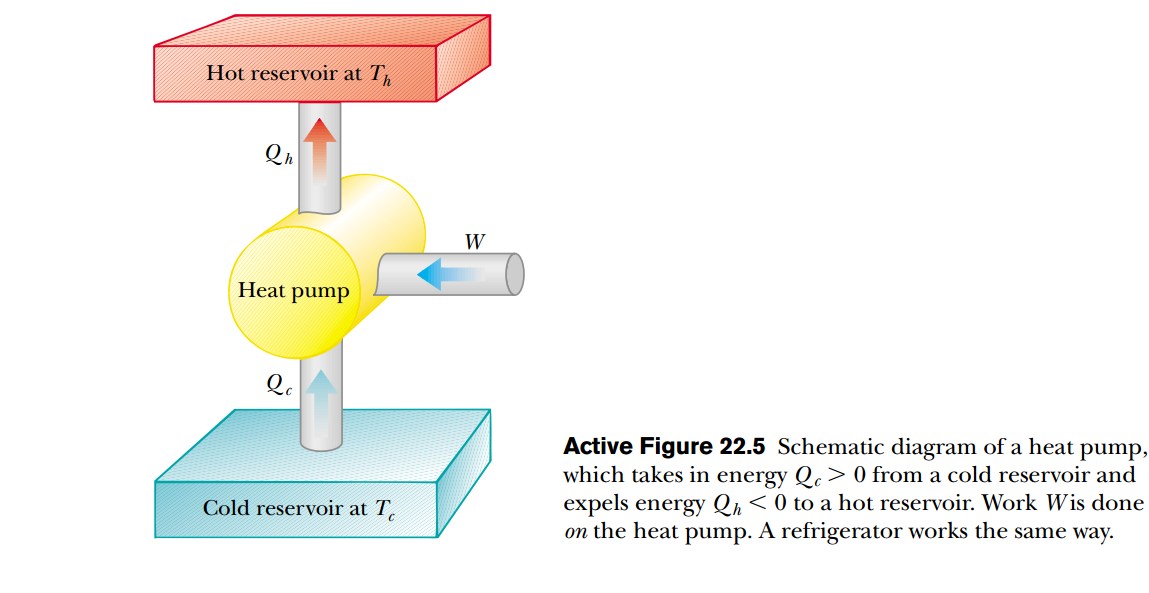
\includegraphics{hinh3}
	- The effectness of heat pump is described as the \textbf{coeficient of performance} (\textbf{COP}).\\ 
	- In the heating mode:
	\begin{mybox}
	\begin{center}
	COP(heating mode) =$\dfrac{\mbox{ energy transferred at high temperature}}{\mbox{ work done by heat pump }} = \dfrac{|Q_{hot}|}{W} > 1 $ 
	\end{center}
	\end{mybox}
	- In the cooling mode:
	\begin{mybox}
	\begin{center}
	COP (cooling mode) = $\dfrac{|Q_{cold}|}{W} > 1?$
	\end{center}
	\end{mybox}
	\textbf{Tip:} $W = \mathscr{P} \times \Delta T$
	%3
	\item \textbf{Reversible and Irreversible Process} (Quá trình thuận nghịch và không thuận nghịch)\\
	 - \textbf{Reversible Process} is the process that the system undergoing can be returned to its initial conditions along the same path on a PV diagram, and every point along this path is an equilibrium state.\\
	 - A process that doesn't satisfy those requirements  is \textbf{Irreversible Process.}
	 %6
	 \item \textbf{The Carnot engine}\\
	 \textit{All the Carnot engine is the reversible process.The engines use Carnot engine have a highest thermal efficiency.}
	 \begin{mybox}
	 \begin{center}
	 $\dfrac{|Q_c|}{|Q_h|} = \dfrac{T_c}{T_h}$
	 \end{center}
	 \end{mybox}
	 The \textbf{Thermal efficiency} of Carnot engine:
	 \begin{mybox}
	 \begin{center}
	 $e_C = 1 - \dfrac{T_c}{T_h}$
	 \end{center}
	 \end{mybox}
	 %5
	 \item \textbf{Entropy} (Độ hỗn loạn)
	 \begin{mybox}
	 \begin{center}
	 dS = $\dfrac{dQ_r}{T}$
	 \end{center}
	 \end{mybox}
	 For T is measured in Kelvin(K).\\
	 \textit{The change in entropy during a process depend only on the end point and therefore is independent of the actual path followed. Consequently, the entropy change for an irreversible process can be determined by calculating the entropy change for a irreversible process that connects the same initial and final states.}\\
	 \textbf{The change in entropy is calculated by:}
	 \begin{mybox}
	 \begin{center}
	 $\Delta S = \displaystyle \int_i^f dS = \int_i^f \dfrac{dQ_r}{T}$
	 \end{center}
	 \end{mybox}
	 \textbf{The total change in entropy in one cycle in a Carnot heat engine:}
	 \begin{mybox}
	 \begin{center}
	 $\Delta S = \dfrac{|Q_h|}{T_h} - \dfrac{|Q_c|}{T_c}$
	 \end{center}
	\end{mybox}
\end{enumerate}
\pagebreak
\begin{center}
\textbf{ELECTRIC CHARGE - ELECTRIC FIELDS }
\end{center}
\textit{ - Electrical \textbf{conductor} (Vật dẫn điện) are materials in which some of the electrons are free electron that are not bound to atoms and can move relatively freely through the material.}\\
\textit{ - Electrical \textbf{insulator} (Vật cách điện) are materials in which all electrons are bound to atoms and cannot move freely through the material.}
\begin{enumerate}
	%1
	\item \textbf{Coulumb's Law}\\
	\textbf{The Properties of the Electric Force:}
	\begin{itemize}
		\item is inversely propotional to the square of the separation \textit{r} between the particles and directed along the line joining them.
		\item is propotional to the product of the charges \textit{$q_1$} and \textit{$q_2$} on the two particle.
		\item is attractive if the charge are of oposite sign and repulsive if the charge have the same sign.
		\item is the conservative force.
	\end{itemize}
	\begin{mybox}
	\begin{center}
	$F_e = k_e \dfrac{|q_1||q_2|}{r^2}$
	\end{center}
	\end{mybox}
	For $k_e = 8.9875 \times 10^9 \approx 9 \times 10^9 N \cdot m^2/C^2$\\
	We have:
	\begin{mybox}
	\begin{center}
	$k_e = \dfrac{1}{4 \pi \epsilon_0}$
	\end{center}
	\end{mybox}
	$\epsilon_0$ is the permittivity of free space.
	\begin{center}
	$\textit{e}_0 = 8.8542 \times 10^{-12} N \cdot m^2 /C^2$
	\end{center}
	The charge on an electron(-e) or a proton (+e) and has a magnitude:
	\begin{center}
	$\textit{e} = 1.60219 \times 10^{-19} C$
	\end{center}
	%2
	\item \textbf{The Electric Field} (Điện trường)\\
	\begin{mybox}
	\begin{center}
	$\textbf{F}_e = q_0 \textbf{E}$
	\end{center}
	\end{mybox}
	For $\textbf{F}_e$ is electric force;\textbf{E} is the electric field.\\
	We have: $\textbf{F}_e = k_e \dfrac{|q||q_0|}{r^2}$.\\
	Then:
	\begin{center}
	$E = k_e \dfrac{|q|}{r^2}$
	\end{center}
	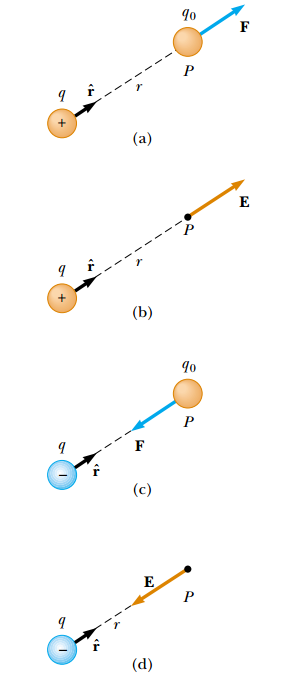
\includegraphics{hinh4}
	%3
	\item \textbf{Electric field of a Continuous Charge Distribution}\\
	- If the charge Q is uniformly distributed throughout a volume V, the \textbf{volume charge density} $\rho$ is defined by:
	\begin{mybox}
	\begin{center}
	$\rho \equiv \dfrac{Q}{V}$
	\end{center}
	\end{mybox}
	- If the charge Q is uniformly distributed on a surface of area A, the \textbf{surface charge density} $\sigma$ is defined by:
	\begin{mybox}
	\begin{center}
	$\sigma \equiv \dfrac{Q}{A}$
	\end{center}
	\end{mybox}
	- If a charge Q is uniformly distributed along a line of length l, the \textbf{linear charge density} $\lambda$ is defined by:
	\begin{mybox}
	\begin{center}
	$\lambda \equiv \dfrac{Q}{l}$
	\end{center}
	\end{mybox}
	%4
	\item \textbf{Electric field line}(Đường sức trường)\\
	\textbf{The rule for drawing electric field lines:}
	\begin{itemize}
	\item The line must begin on a positive charge and terminate on a negative charge.In the case of an excess of one type of charge, some lines will infinitely far away.
	\item The number of lines drawn leaving a positive charge or approaching a negative charge is propotional to the magnitude of the charge.
	\item No two field lines can cross.(Các đường sức trường không cắt nhau)
	\end{itemize}
	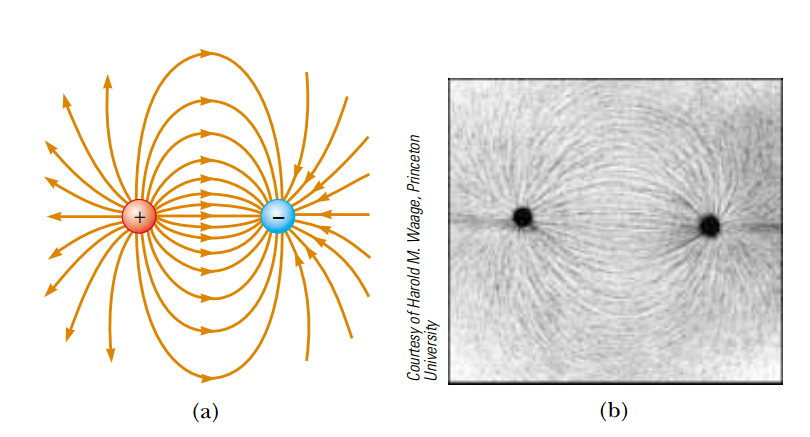
\includegraphics{hinh5}\\
	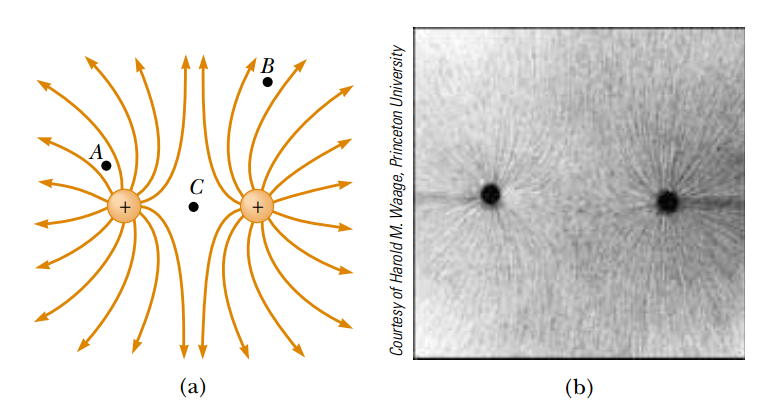
\includegraphics{hinh6}
	%5
	\item \textbf{Motion of Charged Particles in a Uniform Electric Field}\\
	\begin{mybox}
	\begin{center}
	$\textbf{F}_e = q \textbf{E} = m \textbf{a}$
	\end{center}
	\end{mybox}
	The acceleration of the particle is:
	\begin{center}
	$\textbf{a} = \dfrac{q \textbf{E}}{m}$
	\end{center}
\end{enumerate}
\pagebreak
\begin{center}
\textbf{GAUSS'S LAW}
\end{center}
\begin{enumerate}
    %1
    \item \textbf{Electric flux}\\
    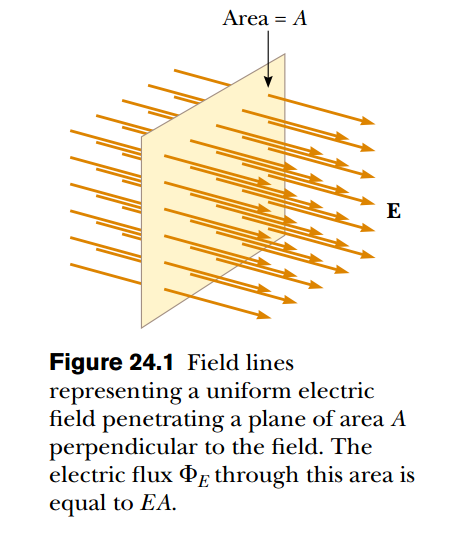
\includegraphics{hinh7}\\
     - Electric flux is propotional to the number of electric field lines penetrating some surface.
     \begin{mybox}
     \begin{center}
     $\Phi_E = EA$
     \end{center}
     \end{mybox}
     - If the surface under consideration is not perpencular to the field,the flux through it will be less than $\phi_E$.\\
     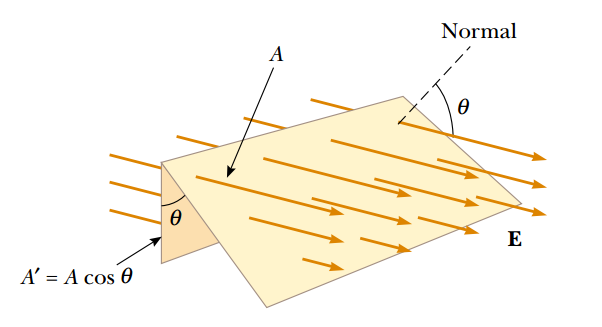
\includegraphics{hinh8}
     \begin{mybox}
     \begin{center}
     $\Phi'_{E} = EA' = EAcos\theta$
     \end{center}
     \end{mybox}
     - In more general situation, we have more than two directions of the surface.Therefore:
     \begin{mybox}
     \begin{center}
     $\Phi_E = \displaystyle \int EdA$
     \end{center}
     \end{mybox}
     - If the area is closed, then we choose $\vec{n}$ outward and $\vec{n}$ is always perpencular to the area.\\
     - The $\vec{n}$ inside the area is always negative, and the $\vec{n}$ outside the area is always positve.\\
     $\rightarrow{\mbox{ The total electric flux of closed area is always zero}}$
     %2
     \item \textbf{Gauss's law} \textit{(The closed surface is consider is gaussian surface or spherical surface)}\\
     - The net flux through the gaussian surface:
     \begin{center}
     $\Phi = \dfrac{k_eq}{r^2} (4 \pi r^2) = 4 \pi k_e q$
     \end{center}
     And: 
     \begin{center}
     $k_e = \dfrac{1}{4 \pi \epsilon_0}$
     \end{center}
     Therefore:
     \begin{center}
     $\Phi_E = \dfrac{q}{\epsilon_0}$
     \end{center}
     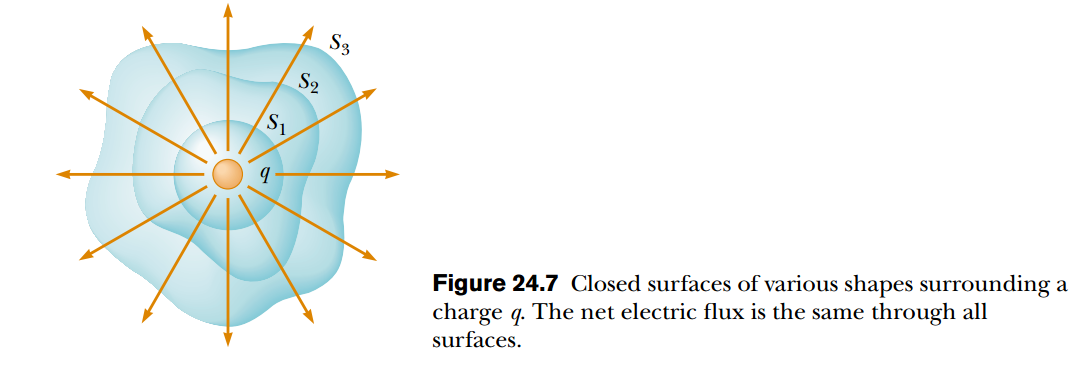
\includegraphics{hinh9}\\
     - The net electric flux through any closed surface surrounding a point charge \textit{q} is given by: $\dfrac{\textbf{q}}{\textbf{$\epsilon_0$}}$ and is independent of the shape of that surface.\\
     - The net electric flux through a closed surface that surround \textbf{no charge} is zero.\\
     - The electric field due to \textbf{many charge} is the vector sum of the electric fields produced by the individual charges.
     \begin{mybox}
     \begin{center}
     $\displaystyle \oint \textbf{$E$} d \textbf{$A$} = \oint (\textbf{$E_1$} + \textbf{$E_2$} + \ldots) \cdot d \textbf{$A$}$
     \end{center}
     \end{mybox}
     - \textbf{Gauss's law}, which is a generalization of what we have just described,states that the net flux through nay closed surface is:
     \begin{mybox}
     \begin{center}
     $\Phi_E = \oint \textbf{$E$} \cdot d\textbf{$A$} = \dfrac{\textbf{$q_{in}$}}{\textbf{$\epsilon_0$}}$
     \end{center}
     \end{mybox}
\end{enumerate} 
\end{document}